% --------------------------------------------------------------
%                           Set Up
% --------------------------------------------------------------
 
\documentclass[12pt]{article}
 
\usepackage[margin=1in]{geometry} 
\usepackage{amsmath,amsthm,amssymb}
\usepackage{listings}
\usepackage{xcolor}
\usepackage{graphicx}
\usepackage{subcaption}
 
\definecolor{codegreen}{rgb}{0,0.6,0}
\definecolor{codegray}{rgb}{0.5,0.5,0.5}
\definecolor{codepurple}{rgb}{0.58,0,0.82}
\definecolor{backcolour}{rgb}{0.95,0.95,0.92}
\definecolor{deepblue}{rgb}{0,0,0.5}
\definecolor{deepred}{rgb}{0.6,0,0}
\definecolor{deepgreen}{rgb}{0,0.5,0}
 
\lstdefinestyle{mystyle}{
    backgroundcolor=\color{backcolour},   
    commentstyle=\color{codegreen},
    keywordstyle=\color{deepred},
    numberstyle=\tiny\color{codegray},
    stringstyle=\color{deepblue},
    basicstyle=\ttfamily\footnotesize,
    breakatwhitespace=false,         
    breaklines=true,                 
    captionpos=b,                    
    keepspaces=true,                 
    numbers=left,                    
    numbersep=5pt,                  
    showspaces=false,                
    showstringspaces=false,
    showtabs=false,                  
    tabsize=2
}
 
\lstset{style=mystyle}
 
\newcommand{\N}{\mathbb{N}}
\newcommand{\Z}{\mathbb{Z}}
 
\newenvironment{theorem}[2][Theorem]{\begin{trivlist}
\item[\hskip \labelsep {\bfseries #1}\hskip \labelsep {\bfseries #2.}]}{\end{trivlist}}
\newenvironment{lemma}[2][Lemma]{\begin{trivlist}
\item[\hskip \labelsep {\bfseries #1}\hskip \labelsep {\bfseries #2.}]}{\end{trivlist}}
\newenvironment{exercise}[2][Exercise]{\begin{trivlist}
\item[\hskip \labelsep {\bfseries #1}\hskip \labelsep {\bfseries #2.}]}{\end{trivlist}}
\newenvironment{problem}[2][Problem]{\begin{trivlist}
\item[\hskip \labelsep {\bfseries #1}\hskip \labelsep {\bfseries #2.}]}{\end{trivlist}}
\newenvironment{question}[2][Question]{\begin{trivlist}
\item[\hskip \labelsep {\bfseries #1}\hskip \labelsep {\bfseries #2.}]}{\end{trivlist}}
\newenvironment{corollary}[2][Corollary]{\begin{trivlist}
\item[\hskip \labelsep {\bfseries #1}\hskip \labelsep {\bfseries #2.}]}{\end{trivlist}}

\newenvironment{solution}{\begin{proof}[Solution]}{\end{proof}}

\setlength\parindent{0pt}
 
\begin{document}
 
% -------------------------------------------------------------- 
%                         Start here
% --------------------------------------------------------------
 
\title{Homework 6}
\author{Timothy Holmes\\ %replace with your name
PHY 440 Classical Mechanics}

\maketitle

\section*{Problem 1}

\subsection*{1a.}

The Lagrangian for this system is given as 

$$
L = \frac{1}{2}m\dot{r}^2 + q\dot{r} \cdot A - q\phi.
$$

The only generalized position in the Lagrangian is $r$ and generalized velocity is $\dot{\dot{r}}$. $r$ can be expanded into $x$, $y$, and $z$ components but for the sake of simplicity $r$ will just be left as $r$ without any loss of information. Thus, the generalized momenta is 

$$
\frac{\partial L}{\partial \dot{q_{i}}} \rightarrow p_{r} = m\dot{r} + q \cdot A.
$$

The Hamiltonian can be found using the following equation

$$
H(\dot{q_{i}}, p_i, t) = \sum_{i = 1}^{n} \dot{q_{i}}p_i - L(\dot{q_{i}}, p_i, t).
$$

Plugging the generalized momenta back into the Hamiltonian the equation becomes 

$$
H(r, \dot{r}, t) = m\dot{r}^{2} + q\dot{r} \cdot A - \frac{1}{2}m\dot{r}^2 + q\dot{r} \cdot A - q\phi
$$

The Hamiltonian can be reduced by combining like terms as such

$$
H(r, \dot{r}, t) = \frac{1}{2}m\dot{r}^2 + q\phi
$$

Writing it in terms of our generalized momenta we can solve for $\dot{r}$ in the generalized momentum equation. Plugging in the results for $\dot{r}$ where $\dot{r} = (p_{r} - q \cdot A)/m$, gives us the Hamiltonian,

$$
H(r, \dot{r}, t) = \frac{1}{2m}(p_{r} - q \cdot A)^{2} + q\phi.
$$

Writing it in this form is important since it allows us to since for Hamilton's equation of motion.

\subsection*{1b.}

The canonical equations of motion for the Hamiltonian are given by

$$
\dot{p_{r}} = -\frac{\partial H}{\partial q_{i}} \rightarrow m\ddot{r} + q\dot{A}
$$

and

$$
\dot{r} = \frac{\partial H}{\partial p_{i}} \rightarrow \frac{1}{m}(p - q \cdot A).
$$

We can rewrite the equation as

$$
m\ddot{r} = -q\Big(\frac{\partial \phi}{\partial r} +\frac{\partial A}{\partial t}\Big) + q \Big[\dot{r}\Big(\frac{\partial A}{\partial x} - \frac{\partial A}{\partial y}\Big) + \dot{r}(\frac{\partial A}{\partial x} - \frac{\partial A}{\partial z}\Big)\Big]
$$

This can be further reduced to 

$$
m\ddot{r} = qE + q[\dot{r}(\nabla_{r} \times A)].
$$

The equation of motion above will finally reduce to 

$$
m\ddot{r} = q[E + \dot{r} \times B].
$$

\subsection*{1c.}

We have the Hamiltonian as,

$$
\dot{p_{r}} = -\frac{\partial H}{\partial q_{i}} \rightarrow m\ddot{r} + q\dot{A}.
$$

When the electric field and magnetic field are zero, that is $E, B(r) = 0$, the $\phi$ component is also zero. Therefore, the Hamiltonian will reduce down to 

$$
H = \frac{1}{2m}|p_{r} - q \cdot A|^{2}.
$$

Since we know that $p_{r} = m\dot{r} + q \cdot A$. We can plug this value into the Hamiltonian such that

$$
H = \frac{d}{dt} \Big[\frac{1}{2m}|m\dot{r}- q \cdot A + q \cdot A |^{2}\Big] \rightarrow H = \frac{d}{dt} \Big[\frac{1}{2m}|m\dot{r} |^{2}\Big] \rightarrow \Big[\frac{d}{dt} \frac{1}{2m} m^{2}\dot{r}^{2}\Big] = 0.
$$

Finally, we can set our velocity term $\dot{r}^{2} = v^{2}$ and one of our mass terms $m$ will cancel out. What out time derivative tells us is that this equation of motion is constant, which leaves us with

$$
\frac{d}{dt}\frac{mv^2}{2} = const.
$$

\subsection*{1d.}

The last problem had the $q\phi$ term drop off since $E = B(r) = 0$. This problem has constant non negative terms where $B = B(r)$ and $E = E_{0}$. Given the Hamiltonian

$$
H = \frac{d}{dt}\Big[\frac{1}{2m}|m\dot{r}- q \cdot A + q \cdot A |^{2} + q\phi\Big].
$$

We can reduce it down like the last equation and set the differentials,

$$
\frac{d}{dt} \Big[\frac{1}{2m}m^{2}\dot{r}^{2} + q\frac{d \phi}{d t}\frac{\partial r}{\partial t} + \frac{\partial \phi}{\partial t}\Big] = 0.
$$

This equation can reduce down to

$$
\frac{d}{dt} \Big[\frac{1}{2}m\dot{r}^{2} + q\frac{d \phi}{d t}\dot{r}\Big] = 0.
$$

Like the previous equation we can set our velocity term $\dot{r}^{2} = v^{2}$ and we get

$$
\frac{d}{dt} \frac{mv^2}{2} = q(E_{0} \cdot \dot{r}).
$$

\section*{Problem 2}

\subsection*{2a.}

The Lagrangian that governs the system for a mass on a vertical rotating hoop is given in the form of

$$
L = \frac{mR^2}{2}(\dot{\theta}^{2} + \omega^{2}sin^2(\theta)) + mgRcos(\theta).
$$

The Hamiltonian can be found using the following equation

$$
H(\dot{q_{i}}, p_i, t) = \sum_{i = 1}^{n} \dot{q_{i}}p_i - L(\dot{q_{i}}, p_i, t).
$$

Since the Lagrangian is given above, the only missing information from the Hamiltonian is the generalized momenta. The generalized momenta is found using 

$$
\frac{\partial L}{\partial \dot{q_{i}}}
$$

The only generalized position in the Lagrangian is $\theta$ and generalized velocity is $\dot{\theta}$. Therefore, the only generalized momenta for the Hamiltonian is 

$$
p_{\theta} = mR^{2}\dot{\theta}.
$$

Plugging the generalized momenta back into the Hamiltonian the equation becomes 

$$
H(\theta, \dot{\theta}, t) = mR^{2}\dot{\theta}^2 - \frac{mR^{2}}{2}\Big(\dot{\theta^{2}} + \omega^{2}sin^{2}(\theta)\Big) - mgRcos(\theta)
$$

The Hamiltonian can be reduced by combining like terms and writing it in terms of our generalized momenta as 

$$
H(\theta, \dot{\theta}, t) = \frac{p_{\theta}^{2}}{2mR^{2}} - \frac{mR^{2}}{2}\Big(\omega^{2}sin^{2}(\theta)\Big) - mgRcos(\theta).
$$

The effective potential for this problem is $U(\theta) = -mR^{2}/2(\omega^{2}sin^{2}(\theta)) + mgRcos(\theta)$. The final Hamiltonian equations becomes

$$
H(\theta, \dot{\theta}, t) = \frac{p_{\theta}^{2}}{2mR^{2}} + U(\theta).
$$

\subsection*{2b.}

The canonical equations of motion for the Hamiltonian are given by

$$
\dot{p_{\theta}} = \frac{\partial H}{\partial \theta} \rightarrow -mR^{2}(\omega^{2}sin(\theta)cos(\theta)) - mgsin(\theta)
$$

and

$$
\dot{\theta} = \frac{\partial H}{\partial p_{\theta}} \rightarrow \frac{p_{\theta}}{mR^2}.
$$

What the canonical equations of the Hamiltonian tell us is that since $p_{\theta} = mR^{2}\dot{\theta}$ then $\ddot{p}_{\theta} = mR^{2}\ddot{\theta}$. Substituting this into the equation above we get 

$$
mR^{2}\ddot{\theta} = -mR^{2}(\omega^{2}sin(\theta)cos(\theta)) - mgRsin(\theta)
$$

This the equation of motion can be reduced into its final for of

$$
\ddot{\theta} = (\omega^{2}cos(\theta) - \frac{g}{R})sin(\theta)
$$

Now, if we are to look at the equilibrium conditions the $cos(\theta)$ and $sin(\theta)$ terms can tell a lot. If we set the equation of motion equal to zero since in the equilibrium condition say the acceleration is zero, then $sin(\theta) = 0$ and $cos(\theta) = g/(R\omega^{2})$. $sin(\theta)$ is zero whenever $\theta = 0$ or $\theta = \pi$, indicating the bead is either at the bottom of the hoop or the top of the hoop. As for $cos(\theta)$ where the equilibrium points are $\theta = \pi/2$ and $\theta = -\pi/2$.


\subsection*{2c.}

Based on the results from above we are plotting $\theta$ vs the function $U(\theta)$. Since $U(\theta)$ components are sinusoidal, we should expect to see some sort of sinusoidal plot. Furthermore, the system is at equilibrium when $\theta$ is constant, leaving $\dot{\theta} = 0$ and $\ddot{\theta} = 0$. Thus, the equilibrium condition is 

$$
sin(\theta)\Big(-\omega^{2}cos(\theta) + \frac{g}{R}\Big) = 0
$$

We are then left with two equilibrium points at $\theta = 0$ when the bead is at the bottom of the hoop or $\theta = \pi$ when the bead is at the top of the hoop as discussed in part b. Based on these two conditions we get the critical rotation rate is 

$$
\omega_{c} = \sqrt{\frac{g}{R}}.
$$

In terms of the critical rotation the equilibrium condition becomes

$$
U(\theta) = \omega^{2}sin(\theta)cos(\theta) + \omega_{c}^{2}sin(\theta).
$$

\begin{figure}[h]
\caption{Plot of $\theta$ vs. $U(\theta)$.}
\centering
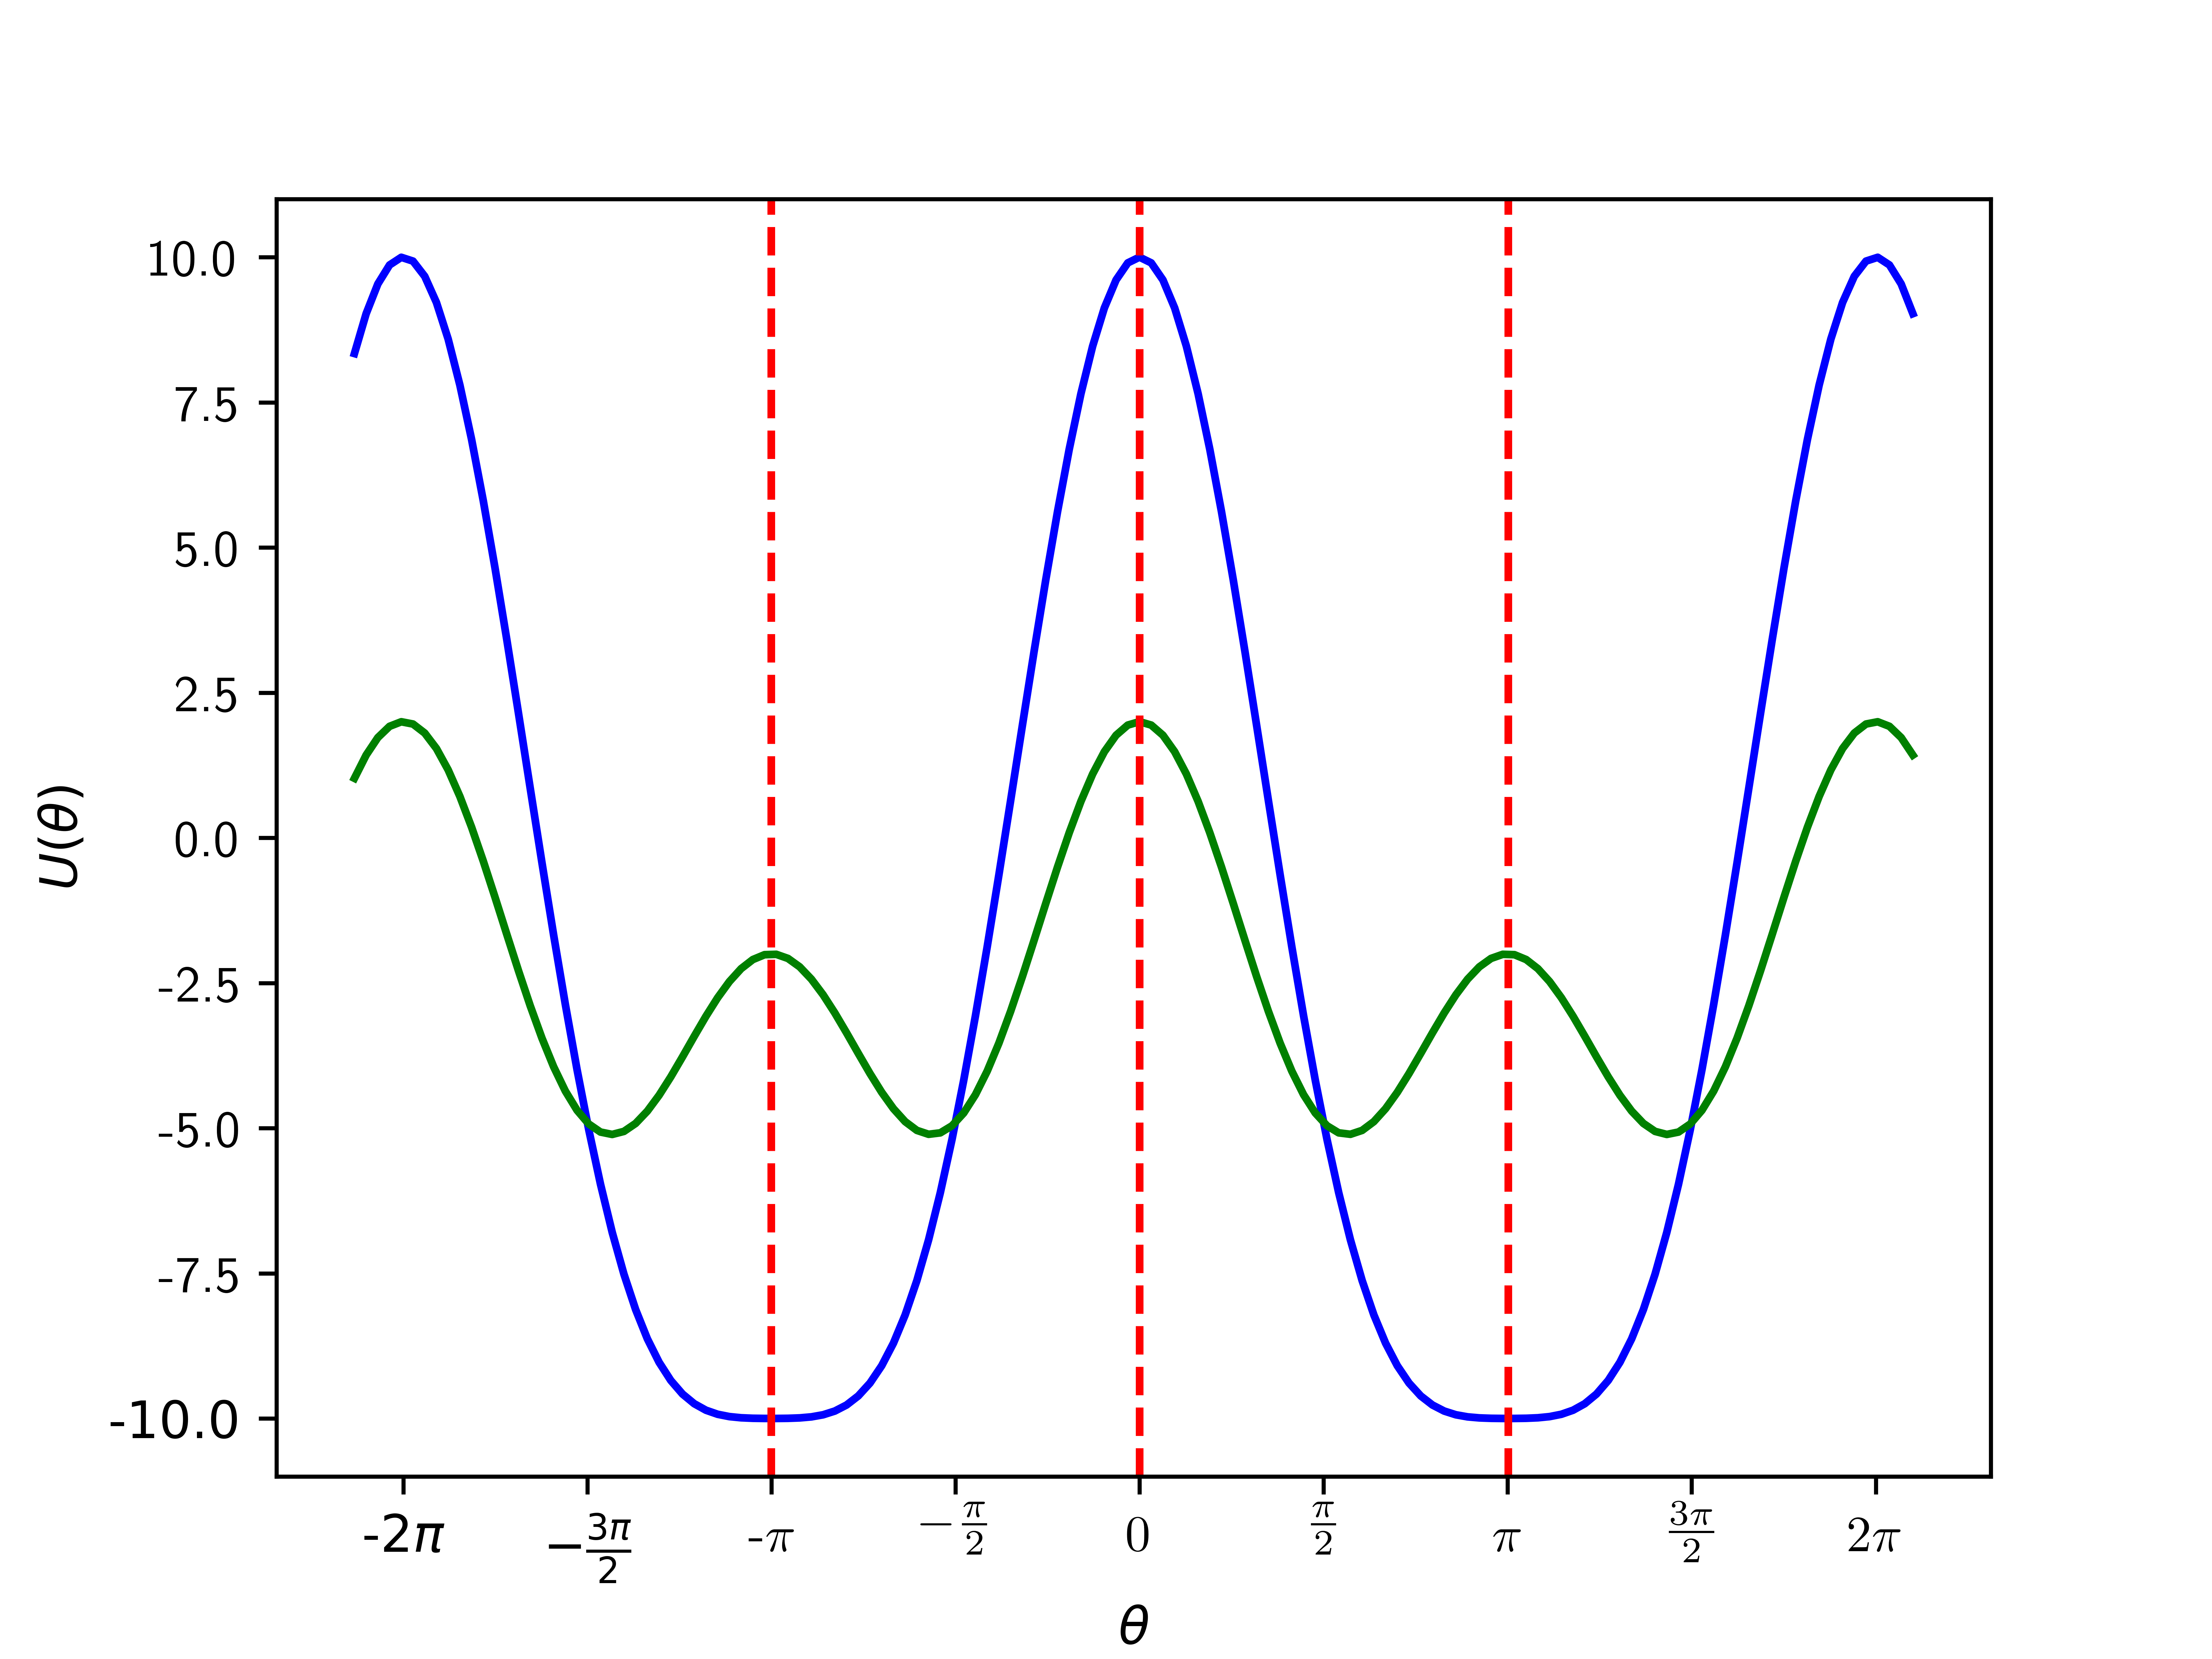
\includegraphics[width=0.75\textwidth]{plot_1.png}
\end{figure}

There are two different plots in Figure 1. The blue line represents $\omega^{2} > g/R$ while the green plot shows that $\omega^{2} < g/R$.

\newpage
\subsection*{2d.}

\begin{figure*}[h]
    \centering
    \begin{subfigure}[t]{0.5\textwidth}
        \centering
        \includegraphics[height=3.5in]{phase_plane_1.png}
        \caption{$\omega^{2} > g/R$}
    \end{subfigure}%
    ~ 
    \begin{subfigure}[t]{0.5\textwidth}
        \centering
        \includegraphics[height=3.5in]{phase_plane_2.png}
        \caption{$\omega^{2} < g/R$}
    \end{subfigure}
    \caption{Phase plane charts where in figure a $\omega^{2} > g/R$ and in figure b $\omega^{2} < g/R$.}
\end{figure*}

Figure 1 compared to the two phase planes in Figure 2 show very similar trends. if we take the scenario where $\omega^{2} > g/R$ i.e. the blue plots, we see in Figure 1 that at $\pi$ and $-\pi$ the plot dips very low ans does not have a hump in it like the green plot. For the same reason the blue plot has a much larger amplitude to it. The blue plot in this case looks more like regular sinusoidal motion than the green plot. In the phase plane we see a dotted circle in the middle, in the green phase plane we see two dotted circles around $\pi/2$ and $\pi$. We see that the green phase plane can never complete a circle a around $0$. Starting clockwise, we see $p$ is steady, decreases, is steady, and then increases. For the green phase plane going clockwise, it increases, decreases, increases, then decreases, increases again, and finally decreases. In Figure 1 we see the same trend in the blue plot going from $-\pi$ to $\pi$. In the same range for the green plot, we see the same trend as just described. But the green plot varies more because of the hump at $-\pi$ and $\pi$.

\newpage
\section*{Appendix}

\begin{lstlisting}[language=Python, caption=Python Graphs]
import numpy as np
import matplotlib.pyplot as plt
import matplotlib as mpl

#---------- Variables -----------
m = 1
R = 1
g = 9.81
omega = np.sqrt(g/R)
omega_c_1 = 10
omega_c_2 = 2
theta = np.arange(-6.7, 6.7, 0.1)

#---------- Figure 1 -----------
U = -(((m * (R ** 2))/2) * ((omega ** 2) * (np.sin(theta) ** 2))
    - (omega_c_1 * np.cos(theta)))

U1 = -(((m * (R ** 2))/2) * ((omega ** 2) * (np.sin(theta) ** 2))
    - (omega_c_2 * np.cos(theta)))

fig, ax = plt.subplots(figsize=(6,4.5))
labels = ax.plot(theta, U,  color='b', linestyle='-')
labels = ax.plot(theta, U1,  color='g', linestyle='-')
pi = ax.axvline(x=3.145, color='r', linestyle='--')
zero = ax.axvline(x=0, color='r', linestyle='--')
neg_pi = ax.axvline(x=-3.145, color='r', linestyle='--')
#ax.legend([labels,neg_pi,zero,pi],bbox_to_anchor=(1.05, 1), loc='upper left', borderaxespad=0.)

mpl.rc('text', usetex = True)
plt.xticks([-2*np.pi, -3*np.pi/2, -np.pi, -np.pi/2, 0, np.pi/2, np.pi, 3*np.pi/2, 2*np.pi],
           [r'-$2\pi$', r'$-\frac{3\pi}{2}$', r'-$\pi$', r'$-\frac{\pi}{2}$', 
           '$0$', r'$\frac{\pi}{2}$', r'$\pi$', r'$\frac{3\pi}{2}$', r'$2\pi$'])

ax.set_xlabel(r'$\theta$')
ax.set_ylabel(r'$U(\theta)$')
plt.savefig('./plot_1.png', dpi=1200)
plt.show()

#---------- Variables -----------
m = 1
R = 1
g = 9.81
omega_c_1 = 10
omega_c_2 = 2
theta = np.arange(-6.7, 6.7, 0.01)
p = np.arange(-6.7, 6.7, 0.01)
Theta, P = np.meshgrid(theta, p)


#---------- Figure 2 -----------
H = ((P ** 2)/(2*m*R**2) - ((m*R ** 2)/2) * (omega ** 2 * np.sin(Theta) ** 2) 
    - omega_c_1 * np.cos(Theta))

fig, ax = plt.subplots(figsize=(6,6))
ax.contour(Theta, P, H, colors='blue')
pi = ax.axvline(x=3.145, color='r', linestyle='--')
zero = ax.axvline(x=0, color='r', linestyle='--')
neg_pi = ax.axvline(x=-3.145, color='r', linestyle='--')

mpl.rc('text', usetex = True)
plt.xticks([-2*np.pi, -3*np.pi/2, -np.pi, -np.pi/2, 0, np.pi/2, np.pi, 3*np.pi/2, 2*np.pi],
           [r'-$2\pi$', r'$-\frac{3\pi}{2}$', r'-$\pi$', r'$-\frac{\pi}{2}$', 
           '$0$', r'$\frac{\pi}{2}$', r'$\pi$', r'$\frac{3\pi}{2}$', r'$2\pi$'])

ax.set_xlabel(r'$\theta$')
ax.set_ylabel(r'$p_{\theta}$')
plt.savefig('./phase_plane_1', dpi=1200)
plt.show()

#---------- Figure 3 -----------
H = ((P ** 2)/(2*m*R**2) - ((m*R ** 2)/2) * (omega ** 2 * np.sin(Theta) ** 2) 
    - omega_c_2 * np.cos(Theta))

fig, ax = plt.subplots(figsize=(6,6))
ax.contour(Theta, P, H, colors='green')
pi = ax.axvline(x=3.145, color='r', linestyle='--')
zero = ax.axvline(x=0, color='r', linestyle='--')
neg_pi = ax.axvline(x=-3.145, color='r', linestyle='--')

mpl.rc('text', usetex = True)
plt.xticks([-2*np.pi, -3*np.pi/2, -np.pi, -np.pi/2, 0, np.pi/2, np.pi, 3*np.pi/2, 2*np.pi],
           [r'-$2\pi$', r'$-\frac{3\pi}{2}$', r'-$\pi$', r'$-\frac{\pi}{2}$', 
           '$0$', r'$\frac{\pi}{2}$', r'$\pi$', r'$\frac{3\pi}{2}$', r'$2\pi$'])

ax.set_xlabel(r'$\theta$')
ax.set_ylabel(r'$p_{\theta}$')
plt.savefig('./phase_plane_2.png', dpi=1200)
plt.show()

\end{lstlisting}


% --------------------------------------------------------------
%                           End Document.
% --------------------------------------------------------------
 
\end{document}
